%%%%%%%%%%%%%%%%%%%%%%%%%%%%%%%%%%%%%%%%%%%%%%%%%%%%%%%%%%%%%%%%%%%%%%%%%%%%%%%%%%%%
\documentclass{article}
\usepackage[margin=1in]{geometry} 
\usepackage{amsmath,amsthm,amssymb,amsfonts, fancyhdr, color, comment, graphicx, environ, float}
\usepackage{mdframed}
\usepackage[shortlabels]{enumitem}
\usepackage{indentfirst}
\usepackage{hyperref}
\hypersetup{
    colorlinks=true,
    linkcolor=blue,
    filecolor=magenta,      
    urlcolor=blue,
}
\usepackage{xcolor}
\usepackage{listings}
\definecolor{mygray}{rgb}{0.8,0.8,0.8}
\lstset{%
    basicstyle=\ttfamily,
    breaklines = true,
    backgroundcolor=\color{mygray},
}
\usepackage{realboxes}
\usepackage{subcaption}

\setlength{\parindent}{0cm}

\pagestyle{fancy}

% \newenvironment{problem}[2][Problem]
%     { \begin{mdframed}[backgroundcolor=gray!20] \textbf{#1 #2} \\}
%     {  \end{mdframed}}

% % Define solution environment
% \newenvironment{solution}{\noindent\textbf{Solution}}

%%%%%%%%%%%%%%%%%%%%%%%%%%%%%%%%%%%%%%%%%%%%%
%Fill in the appropriate information below
\lhead{Jakob Johnson, u0972673}
\rhead{CS 6350 - Machine Learning} 
\chead{\textbf{Mid-Term Project Report}}
%%%%%%%%%%%%%%%%%%%%%%%%%%%%%%%%%%%%%%%%%%%%%


\begin{document}
    The code is mentioned in this report is available on \href{https://github.com/jakobottar/2021-ml-project}{GitHub}.

    \section{AdaBoost}
        I first tried to fit the model with AdaBoost. I suspected that a simple decision tree would not do well, and even if so AdaBoost should do approximately as well. I chose to try the \lstinline{sklearn} implementation \lstinline{sklearn.ensemble.AdaBoostClassifier}. This implementation requires a feature array and a result array that are all numeric, so I had to read in the data with \lstinline{pandas} and perform feature mapping to convert the string-formatted categorical variables to numeric variables that could be read by the AdaBoost classifier.  \\

        After formatting the data I wanted to determine the best number of classifiers to include in my AdaBoost model so I ran 5-fold cross-validation on models using 1 to 750 (skipping every 10) classifiers. I stored the number of classifiers that got the highest accuracy and then plotted the accuracy (figure \ref{fig:ab_acc}). We achieved a max training accuracy of approximately 87\%.
        \begin{figure}[H]
            \centering
            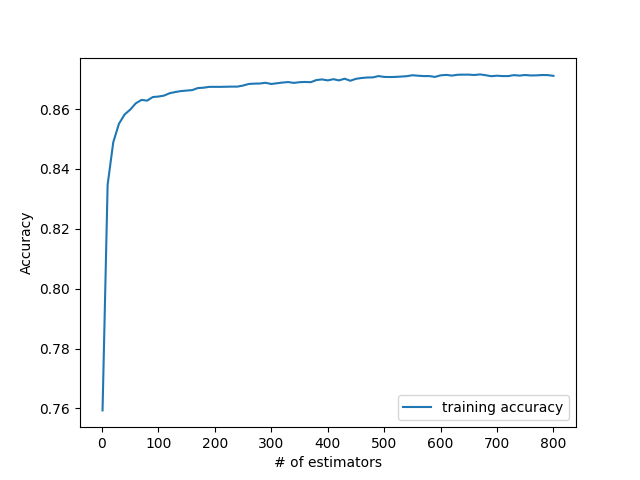
\includegraphics[width=0.5\linewidth]{./img/ab_acc.png}
            \caption{AdaBoost accuracy versus number of classifiers used.}
            \label{fig:ab_acc}
        \end{figure}

        In the end I used the max, 750 classifiers, to train the final model using all the training data. I could potentially continue to increase the number of classifiers, but the model takes quite a bit of time to train at 750 and that only showed marginal gains over models using 300 and 500 estimators. \\

        After training the model I formatted the testing set the same way as the training set, converting categorical variables to numeric, and used the fully-trained model to predict the \lstinline{'income>50K'} attribute for each value. Saving this as a csv and uploading to Kaggle showed an accuracy of 73.041\%. 

    \section{Random Forests}
        After trying AdaBoost and getting a decent result, I decided to try the similar method Random Forests. Since Random Forests are more robust to overfitting and since we got a training accuracy of 87\% and a testing accuracy of only 73\%, I think that the model might be overfitting too much. I again chosethe \lstinline{sklearn} implementation \lstinline{sklearn.ensemble.RandomForestClassifier}. Similarly to \lstinline{AdaBoostClassifier}, this implementation requires a feature array and a result array that are all numeric, so I had to read in the data with \lstinline{pandas} and perform feature mapping to convert the string-formatted categorical variables to numeric variables that could be read by the Random Forest classifier.  \\

        After formatting the data I again wanted to determine the best number of classifiers to include in my Random Forest model so I ran 5-fold cross-validation on models using 1 to 750 (skipping every 10) classifiers. I stored the number of classifiers that got the highest accuracy and then plotted the accuracy (figure \ref{fig:rf_acc}). We achieved a max training accuracy of approximately 86\%, slightly lower than that of AdaBoost. 
        \begin{figure}[H]
            \centering
            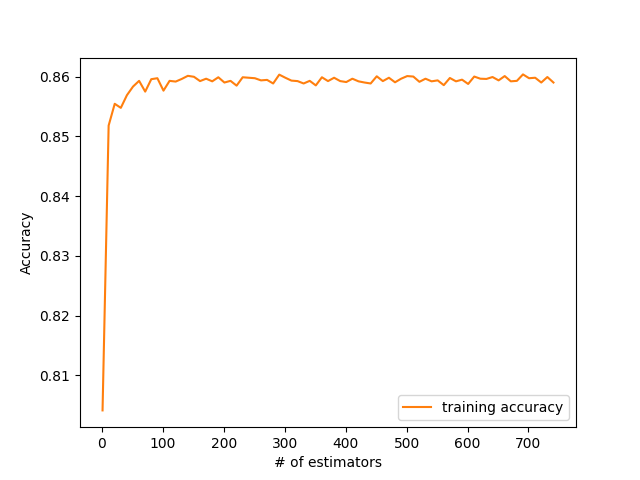
\includegraphics[width=0.5\linewidth]{./img/rf_acc.png}
            \caption{Random Forest accuracy versus number of classifiers used.}
            \label{fig:rf_acc}
        \end{figure}

        In the end I again used the max, 750 classifiers, to train the final model using all the training data. \\

        After training the model I formatted the testing set the same way as the training set, converting categorical variables to numeric, and used the fully-trained model to predict the \lstinline{'income>50K'} attribute for each value. Saving this as a csv and uploading to Kaggle showed an accuracy of 77.197\%, slightly higher than that of AdaBoost, confirming my hypothesis that the AdaBoost model was overfitting and Random Forest's robustness to that would lead to a higher testing accuracy.
    
    \section{Support Vector Machines}
        I breifly tried using Support Vector Machines, using the \lstinline{sklearn.svm.SVC} implementation, however it was very very slow, taking 20+ minutes to train on the training set. I might attempt this in the future however I think I will still run into performance issues and my time might be better spent on more powerful methods.

    \section{Future Work}
        For the rest of the project, I think I can get much higher accuracy (some students have already hit 90+\% accuracy on the leaderboards) using neural nets. This is where I will focus much of my time, tuning and refining an architecture. I also plan on exploring some simpler methods we will discuss in class such as Nearest-Neighbors and Naive Bayes algorithms. \\

        I will also do some more exploratory data analysis, plotting and analyzing the data visually and numerically. This has helped me significantly in the past by refining the scope of models to try as well as potentially providing some insight into data agumentation or new feature combinations to try.


\end{document}

% \begin{figure}[H]
%     \centering
%     \begin{subfigure}{0.4\textwidth}
%         \includegraphics[width=\linewidth]{./img/1.png} 
%         \caption{1}
%     \end{subfigure}
%     \begin{subfigure}{0.4\textwidth}
%         \includegraphics[width=\linewidth,]{./img/2.png}
%         \caption{2}
%     \end{subfigure}
%     \begin{subfigure}{0.4\textwidth}
%         \includegraphics[width=\linewidth]{./img/3.png} 
%         \caption{3}
%     \end{subfigure}
%     \begin{subfigure}{0.4\textwidth}
%         \includegraphics[width=\linewidth,]{./img/4.png}
%         \caption{4}
%     \end{subfigure}

%     \caption{Examples of images}
% \end{figure}
